\documentclass[12pt, letterpaper]{article}
\usepackage{multirow}
\usepackage{graphicx}
\usepackage[letterpaper, margin=1in]{geometry}



\begin{document}

\section*{Curved Mesh Generation}

	\begin{tabular}{|c|c|c|c|}
		\hline
		& Coarse & Medium & Fine \\
		\hline
		No. of points 				& 32,841 & 243,729	& 1,875,489 \\
		No. of boundary points		& 2,304	& 8,704		& 33,792 \\
		Support radius				& 0.06	& 0.06		& 0.04 \\
		Minimum scaled Jacobian	& 0.714	& 0.852		& 0.926 \\
		Wall-clock time			& 0.68s	& 12.6s		& 338s \\
		\hline
	\end{tabular}
	
	Summary of 3D bump curved mesh generation
	\vspace{0.5in}

	\begin{tabular}{|c|c|c|c|c|}
		\hline
		Method & Parameters & Min. scaled Jacobian & Wall clock time & Solver iterations \\
		\hline
		\multirow{2}{0.5in}{SLE} & $\chi=2.75$ & 0.632 & 19.3s & 324 \\
		& $\chi=2.9$ & 0.632 & 24.4s & 423 \\
		\multirow{3}{0.5in}{RBF} & 1-step $r_s=0.04$ & 0.640 & 1.86s & 365 x 2 \\
		&   1-step $r_s=0.08$ & 0.639 & 1.9s & 1150 x 2\\
		&   2-step $r_s=0.04$ & 0.641 & 2.58s & 365 x 4\\
		\hline
	\end{tabular}
	
	Comparison of RBF (radial basis function) and SLE (stiffened linear elasticity) methods

\begin{figure}[!h]
	\flushleft
	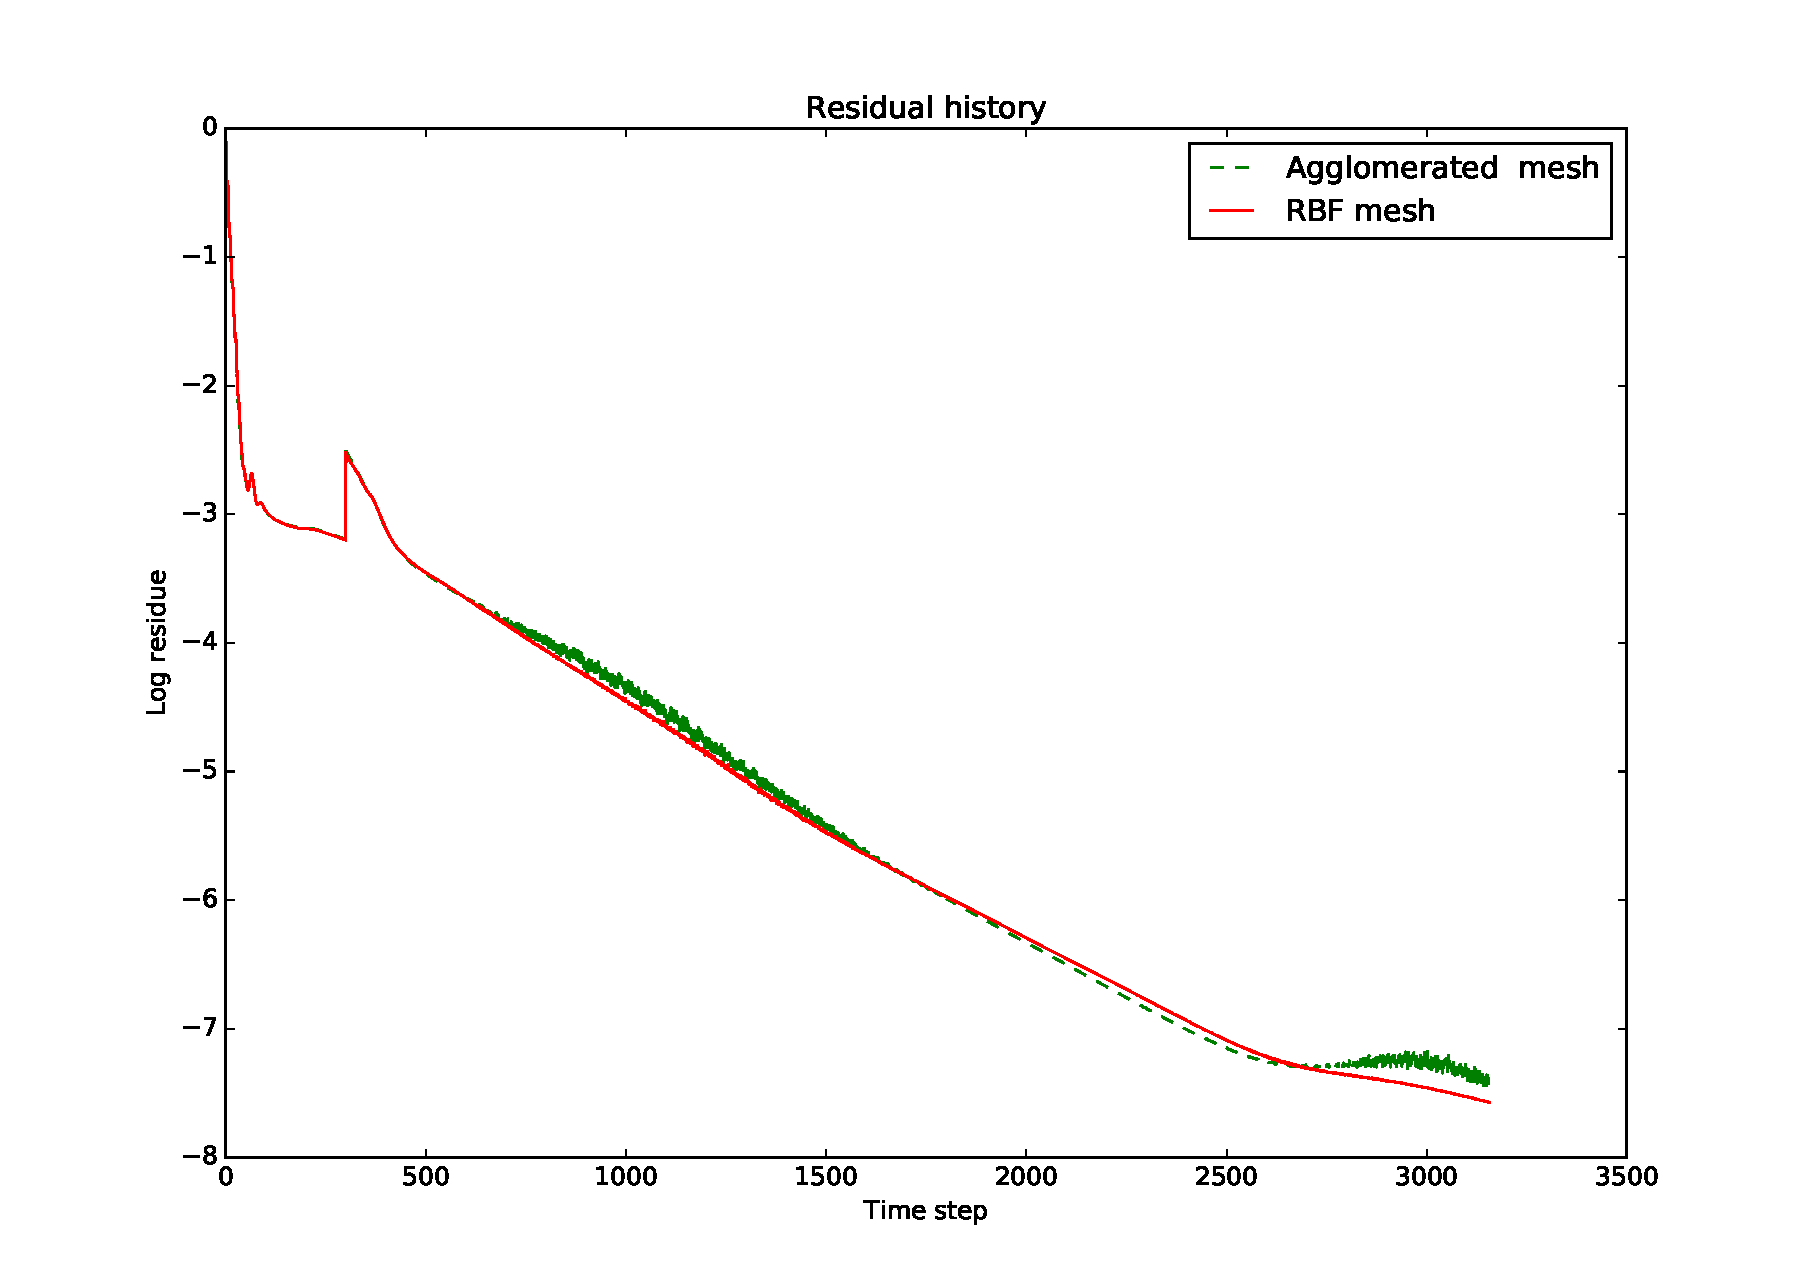
\includegraphics[scale=0.6]{solver-convergence}
	\caption{Comparison of residual convergence history with time steps for implicit DG P1 solution}
\end{figure}
\end{document}
